\documentclass[tikz,border=3pt]{standalone}
\usetikzlibrary{arrows.meta,positioning}
\definecolor{textcolor}{HTML}{0F172A}
\definecolor{muted}{HTML}{475569}
\definecolor{panel}{HTML}{F8FAFC}
\definecolor{edgecolor}{HTML}{334155}
\definecolor{risklowcolor}{HTML}{10B981}
\definecolor{riskmediumcolor}{HTML}{F59E0B}
\definecolor{riskhighcolor}{HTML}{F43F5E}
\definecolor{riskcriticalcolor}{HTML}{BE123C}
\definecolor{riskunknowncolor}{HTML}{94A3B8}
\tikzset{
  base/.style={rounded corners=2pt, align=center, draw=edgecolor, line width=0.45pt, inner sep=3.0pt, font=\sffamily\scriptsize, text=textcolor},
  context/.style={base, fill=cyan!12, draw=cyan!55!black, minimum width=2.05cm, minimum height=0.72cm},
  decision/.style={base, fill=blue!12, draw=blue!70!black, minimum width=2.45cm, minimum height=0.82cm},
  risklow/.style={base, fill=risklowcolor, draw=white, text=white, minimum width=2.95cm, minimum height=0.82cm},
  riskmedium/.style={base, fill=riskmediumcolor, draw=white, text=white, minimum width=2.95cm, minimum height=0.82cm},
  riskhigh/.style={base, fill=riskhighcolor, draw=white, text=white, minimum width=2.95cm, minimum height=0.82cm},
  riskcritical/.style={base, fill=riskcriticalcolor, draw=white, text=white, minimum width=2.95cm, minimum height=0.82cm},
  riskunknown/.style={base, fill=riskunknowncolor, draw=white, text=white, minimum width=2.95cm, minimum height=0.82cm},
  evidence/.style={base, fill=white, draw=gray!25, minimum width=5.20cm, text width=4.90cm, minimum height=0.96cm},
  outcome/.style={base, fill=red!8, draw=red!45, minimum width=1.75cm, minimum height=0.70cm, font=\sffamily\scriptsize},
  edge/.style={-Latex, draw=edgecolor, line width=0.55pt},
  thinflow/.style={-Latex, draw=edgecolor, opacity=0.42, line width=0.36pt},
}
\begin{document}
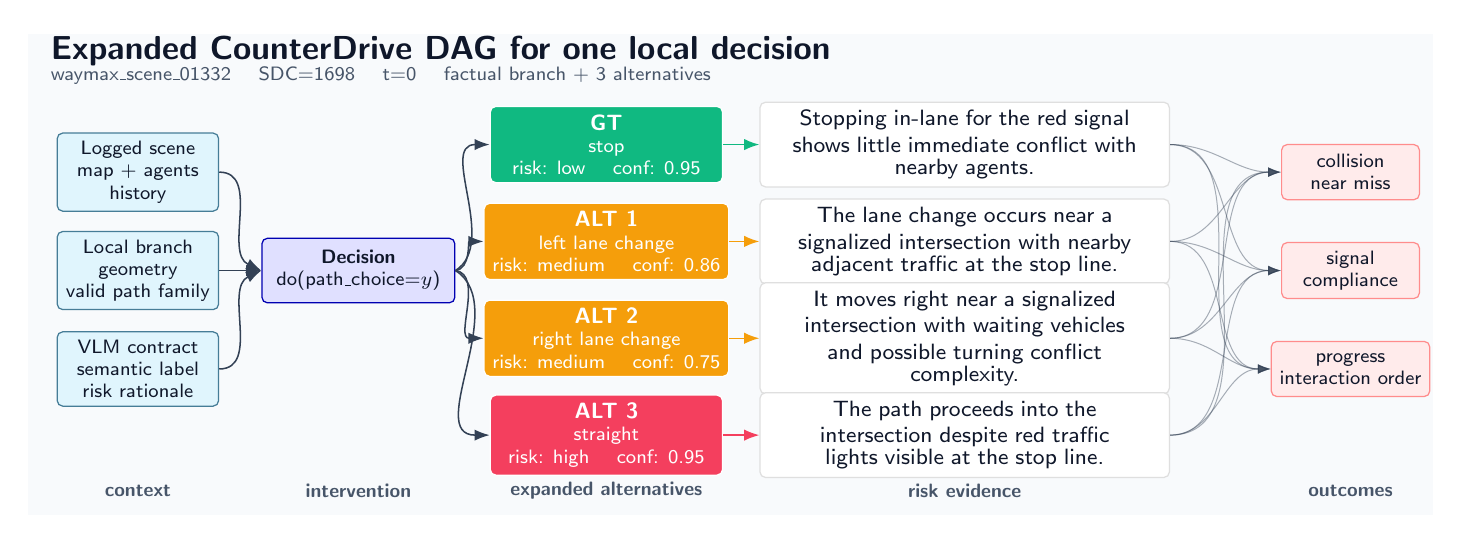
\begin{tikzpicture}[x=1cm,y=1cm]
  \fill[panel] (-0.35,0.35) rectangle (17.50,6.45);

  \node[anchor=west, font=\sffamily\bfseries\large, text=textcolor] at (-0.18,6.23)
    {Expanded CounterDrive DAG for one local decision};
  \node[anchor=west, font=\sffamily\scriptsize, text=muted] at (-0.18,5.93)
    {waymax\_scene\_01332 \quad SDC=1698 \quad t=0 \quad factual branch + 3 alternatives};

  \node[context] (scene) at (1.05,4.70) {Logged scene\\ map + agents\\ history};
  \node[context] (branch) at (1.05,3.45) {Local branch\\ geometry\\ valid path family};
  \node[context] (contract) at (1.05,2.20) {VLM contract\\ semantic label\\ risk rationale};

  \node[decision] (decision) at (3.85,3.45) {\textbf{Decision}\\ do(path\_choice=$y$)};

  \draw[edge] (scene.east) to[out=0,in=155] (decision.west);
  \draw[edge] (branch.east) -- (decision.west);
  \draw[edge] (contract.east) to[out=0,in=205] (decision.west);

\node[risklow] (slot0) at (7.00,5.05) {\footnotesize\textbf{GT}\\ stop\\ \scriptsize risk: low \quad conf: 0.95};
\node[riskmedium] (slot1) at (7.00,3.82) {\footnotesize\textbf{ALT 1}\\ left lane change\\ \scriptsize risk: medium \quad conf: 0.86};
\node[riskmedium] (slot2) at (7.00,2.59) {\footnotesize\textbf{ALT 2}\\ right lane change\\ \scriptsize risk: medium \quad conf: 0.75};
\node[riskhigh] (slot3) at (7.00,1.36) {\footnotesize\textbf{ALT 3}\\ straight\\ \scriptsize risk: high \quad conf: 0.95};

\node[evidence] (risk0) at (11.55,5.05) {\footnotesize Stopping in-lane for the red signal\\ shows little immediate conflict with\\ nearby agents.};
\node[evidence] (risk1) at (11.55,3.82) {\footnotesize The lane change occurs near a\\ signalized intersection with nearby\\ adjacent traffic at the stop line.};
\node[evidence] (risk2) at (11.55,2.59) {\footnotesize It moves right near a signalized\\ intersection with waiting vehicles\\ and possible turning conflict\\ complexity.};
\node[evidence] (risk3) at (11.55,1.36) {\footnotesize The path proceeds into the\\ intersection despite red traffic\\ lights visible at the stop line.};

\draw[edge] (decision.east) to[out=32,in=180] (slot0.west);
\draw[edge] (decision.east) to[out=8,in=180] (slot1.west);
\draw[edge] (decision.east) to[out=-8,in=180] (slot2.west);
\draw[edge] (decision.east) to[out=-32,in=180] (slot3.west);

\draw[edge, draw={risklowcolor}] (slot0.east) -- (risk0.west);
\draw[edge, draw={riskmediumcolor}] (slot1.east) -- (risk1.west);
\draw[edge, draw={riskmediumcolor}] (slot2.east) -- (risk2.west);
\draw[edge, draw={riskhighcolor}] (slot3.east) -- (risk3.west);

  \node[outcome] (collision) at (16.45,4.70) {collision\\ near miss};
  \node[outcome] (compliance) at (16.45,3.45) {signal\\ compliance};
  \node[outcome] (progress) at (16.45,2.20) {progress\\ interaction order};

\draw[thinflow] (risk0.east) to[out=0,in=180] (collision.west);
\draw[thinflow] (risk0.east) to[out=0,in=180] (compliance.west);
\draw[thinflow] (risk0.east) to[out=0,in=180] (progress.west);
\draw[thinflow] (risk1.east) to[out=0,in=180] (collision.west);
\draw[thinflow] (risk1.east) to[out=0,in=180] (compliance.west);
\draw[thinflow] (risk1.east) to[out=0,in=180] (progress.west);
\draw[thinflow] (risk2.east) to[out=0,in=180] (collision.west);
\draw[thinflow] (risk2.east) to[out=0,in=180] (compliance.west);
\draw[thinflow] (risk2.east) to[out=0,in=180] (progress.west);
\draw[thinflow] (risk3.east) to[out=0,in=180] (collision.west);
\draw[thinflow] (risk3.east) to[out=0,in=180] (compliance.west);
\draw[thinflow] (risk3.east) to[out=0,in=180] (progress.west);

  \node[font=\sffamily\scriptsize\bfseries, text=muted] at (1.05,0.65) {context};
  \node[font=\sffamily\scriptsize\bfseries, text=muted] at (3.85,0.65) {intervention};
  \node[font=\sffamily\scriptsize\bfseries, text=muted] at (7.00,0.65) {expanded alternatives};
  \node[font=\sffamily\scriptsize\bfseries, text=muted] at (11.55,0.65) {risk evidence};
  \node[font=\sffamily\scriptsize\bfseries, text=muted] at (16.45,0.65) {outcomes};
\end{tikzpicture}
\end{document}
